\section{Drakonia}\label{drakonia}

Tags: Stato Creatore: Lorenzo

\section{Drakonia}\label{drakonia-1}

\begin{center}\rule{0.5\linewidth}{0.5pt}\end{center}

\begin{figure}
\centering
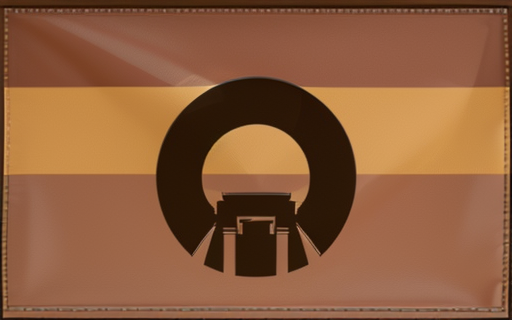
\includegraphics{flag_(2).png}
\caption{flag (2).png}
\end{figure}

Informazioni Generali

Nome Ufficiale: Drakonia

Lingue Ufficiali: Comune Valtarese

Capitale: La Cittadella

Forma di Governo: Dittatura Totalitaria

Popolazione: N.A.

Superficie:

Continente: Valtara

Alleati:

\begin{center}\rule{0.5\linewidth}{0.5pt}\end{center}

\subsection{1. Descrizione Generale}\label{descrizione-generale}

\begin{center}\rule{0.5\linewidth}{0.5pt}\end{center}

Drakonia è un regno cupo e misterioso, situato sul delta del fiume
Kratos lungo la costa. La sua imponente capitale, la cittadella, è
circondata da alte mura impenetrabili. La popolazione vive sotto il
controllo assoluto del Re Oscuro. Il governo è totalitario.

\subsection{2. Storia}\label{storia}

\begin{center}\rule{0.5\linewidth}{0.5pt}\end{center}

Nell'anno 1032, Draco Valerian, era il delfino della nobile casata reale
del Drakodor. Tuttavia, quel periodo rimane impresso nella memoria
collettiva come l'anno della Piaga, un evento climatico devastante che
gettò le fertili terre di Valtara nell'abisso della crisi. Le colture
languirono, le malattie mietevano vite e le autorità statali si
sgretolavano sotto il peso della catastrofe. Il regno di Drakondor, in
pochi anni, subì un declino irreversibile. La popolazione si ridusse
drammaticamente a causa delle malattie e della carestia, mentre chi
poteva fuggì verso regioni non ancora colpite dalla Piaga. Tra i membri
della famiglia reale, solo Draco sopravvisse alla tragedia, seppur
privato delle ricchezze che la sua casata aveva speso per fronteggiare
la crisi. Abbandonato, il giovane principe divenne un vagabondo, privo
di qualsiasi segno distintivo della sua precedente nobiltà. Il suo
regno, una volta glorioso, crollò rapidamente sotto i colpi del destino.
Vagabondando per le terre di Valtara, Draco, pur sconfitto, covava il
desiderio ardente di restaurare l'antico splendore di Drakodor, un regno
maestoso destinato a dominare l'intera penisola. Avrebbe concesso
l'anima ad un demone per poter rivedere il suo regno splendere ancora, e
così fece. Fu in questo momento di vulnerabilità che incrociò la strada
di un demone, che seducente gli prometteva un potere incommensurabile,
con il quale avrebbe potuto raccogliere tra le sue mani anche il mondo
intero se solo lo avesse desiderato. Draco accolse con incoscente
felicità l'offerta, cadendo così in un tormentato e lento oblio,
permettendo al demone di nutrirsi della sua anima. Nessuno conosce cosa
avvenì realmente, in che modo il demone si servì di lui, ma dopo più di
otto secoli di oscurità, Draco emerse come un Lich potente e imponente,
deciso a riconquistare ciò che considerava suo di diritto. Ricostituire
il regno di Drakondor divenne l'obiettivo della sua implacabile
vendetta. Un conflitto sanguinoso, noto tra gli annali come la Guerra
del Kratos, infiammò la penisola di Valtara per anni (1914-1918), mentre
Draco, seguito da un esercito demoniaco, cercava di ristabilire il suo
dominio sulle fertili terre del delta del Kratos. Da ogni angolo di
Valtara gli eserciti si riversarono nella regione del Drakon, unendosi
in un fronte comune per contrastare la terribile avanzata delle forze
del male, incarnate nel Lich che lasciava morte ovunque passasse. La
guerra non fu persa, ma neanche vinta. Draco riuscì a stabilire il
proprio dominio sulle fertili terre del delta del Kratos, antico cuore
del suo regno perduto. Nacque così il regno di Drakonia, una spietata
monarchia assoluta, dove il Re Oscuro governava con mano inflessibile,
tenendo in ostaggio i popoli di quelle terre. Dopo 10 anni dalla
conquista di quei territori, parte del regno venne sfollato, e separato
dal mondo esterno da imponenti mura di pietra, dietro le quali si cela
l'ignoto. Il resto del paese, libero da barriere fisiche, venne invece
invaso da creature demoniache, il cui compito era, ed è, quello di
proteggere i confini del regno. Dopo di ciò nessun'altra notizia
pervenne dal regno di Drakonia, ormai immobile da più di un secolo.

\subsection{3. Geografia}\label{geografia}

\begin{center}\rule{0.5\linewidth}{0.5pt}\end{center}

\begin{figure}
\centering
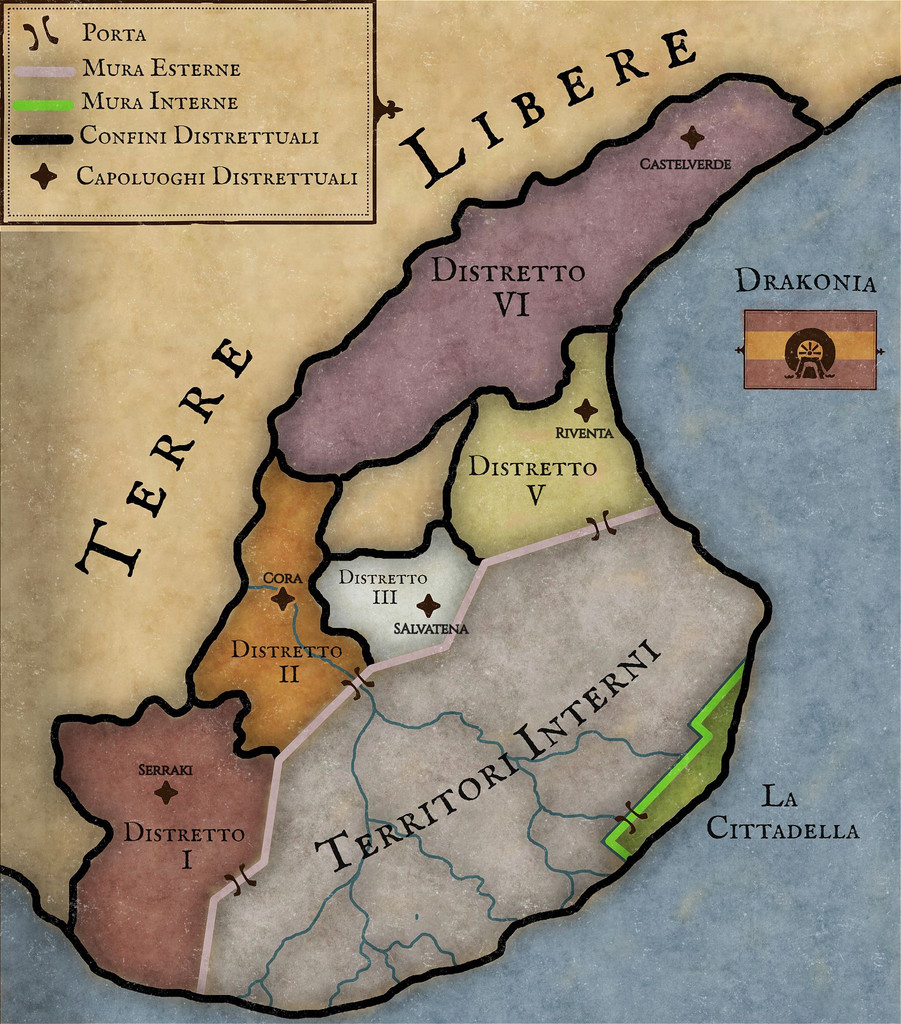
\includegraphics{immafin.jpg}
\caption{immafin.jpg}
\end{figure}

La terra stessa su cui poggia questo regno spettrale è il vasto delta
del fiume Kratos. Sulla costa di questa terra minacciosa sorge la sua
imponente capitale, la Cittadella, circondata da maestose mura che
celano il vero aspetto della città. Nessuno conosce cosa realmente
succede nella cittadella, ne conosce il suo aspetto: la capitale è stata
costruita alla fine della guerra, e fin da subito è stata nascosta dalle
sue mura. I territori interni, un tempo rigogliosi e fertili grazie alle
acque del Kratos, sono ora segregati dal resto del mondo da un muro
impenetrabile, un'ombra fisica della desolazione interiore che ha
avvolto il regno. Ciò che accade dietro quelle difese impenetrabili
rimane un enigma, lasciando spazio solo a congetture e aleggiando nel
territorio dell'ignoto. Si ipotizza che i territori interni, che
separano i distretti dalla cittadella, siano completamente inutilizzati,
poichè i suoi abitanti vennero sfollati prima della costruzione delle
mura.

I distretti esterni agiscono come una sorta di zona cuscinetto tra il
regno e il mondo esterno, come avamposti in cui l'oscurità di Drakonia
si scontra con la luce esterna. In questi 5 distretti la vita scorre
quasi allo stesso modo che nel resto di Valtara, i commerci con
l'esterno sono ammessi e l'economia della zona non è succube della
cittadella. Ma anche qui, il velo dell'incertezza e della paura si
adagia su ogni centimetro di terreno, poiché il regno spettrale tiene
saldamente le redini di questi confini, esercitando un oppressivo
controllo militare su tutta la popolazione, e su tutto ciò che può
entrare e uscire. I distretti esterni sono i seguenti:

\begin{itemize}
\tightlist
\item
  Distretto I o Distretto di Serraki
\item
  Distretto II o Distretto di Cora
\item
  Distretto III o Distretto di Salvatena
\item
  Distretto IV: Non più esistente. È stato distrutto per impartire una
  lezione ai distretti alla fine della Guerra. Ad oggi le terre del
  distretto IV sono ancora abbandonate.
\item
  Distretto V o Distretto di Riventa
\item
  Distretto VI o Distretto di Castelverde
\end{itemize}

\subsection{4. Demografia}\label{demografia}

\begin{center}\rule{0.5\linewidth}{0.5pt}\end{center}

Non abbiamo dati a sufficienza per un'esaustiva analisi della demografia
del regno. Non conosciamo neanche l'esatto numero di abitati. Tuttavia,
nei distretti la popolazione è molto eterogenea, e riflette la
situazione demografica della Valtara.

\subsection{5. Economia}\label{economia}

\begin{center}\rule{0.5\linewidth}{0.5pt}\end{center}

L'economia di Drakonia, sebbene avvolta in un velo di mistero, si basa
principalmente su un sistema di sfruttamento e di oppressione. Le
risorse del regno, una volta abbondanti e produttive, ora vengono
sfruttate a vantaggio del Re. Gran parte di ciò che viene prodotto nei
distretti esterni viene destinato alla Cittadella, e i cittadini dei
distretti sono privati di qualsiasi possibilità di prosperità personale.

Il commercio esterno è limitato, ma possibile solo nei distretti
esterni.

\subsection{6. Cultura}\label{cultura}

\begin{center}\rule{0.5\linewidth}{0.5pt}\end{center}

Le espressioni culturali del popolo dei distretti è in linea con quelle
dei vicini territori liberi, ma vengono pesantemente limitate.

\subsection{7. Governo}\label{governo}

\begin{center}\rule{0.5\linewidth}{0.5pt}\end{center}

Il governo di Drakonia si erge come una struttura totalitaria e
autocratica, con il Re Lich che detiene un potere assoluto e indiscusso
su ogni aspetto della vita all'interno del regno. Le decisioni politiche
e amministrative sono prese senza alcuna forma di consultazione o
consenso popolare, e le leggi stesse è un riflesso delle volontà e degli
ordini del sovrano spettrale.

Una fitta rete di servitori e funzionari devoti implementa la sua
volontà con fermezza e senza pietà. Tra tutti i suoi servitori, i più
spietati sono i 4 Cavalieri: figure oscure, di cui nessuno conosce la
vera identità. Vengono considerati gli occhi e le orecchie del Re, e
vagano per il regno assicurandosi che la legge di Drakonia venga
rispettata. Agiscono secondo diretto volere del Re, e ogni loro
decisione viene considerata legge.

\begin{figure}
\centering
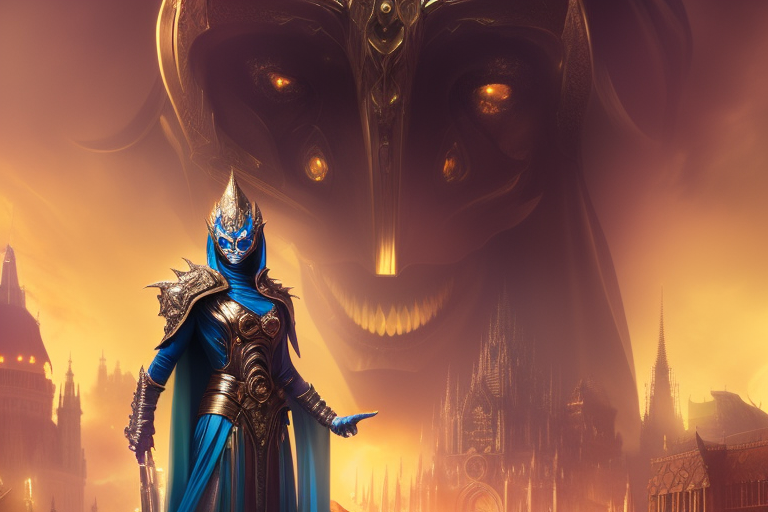
\includegraphics{lich_e_cazzi.png}
\caption{I quattro Cavalieri celano la propria identità dietro le loro
vesti azzurre e le armature dorate. Ognuno di loro esegue la volontà del
potente Re Oscuro}
\end{figure}

I quattro Cavalieri celano la propria identità dietro le loro vesti
azzurre e le armature dorate. Ognuno di loro esegue la volontà del
potente Re Oscuro

Ogni forma di opposizione è soffocata nel suo guscio, con un apparato di
sicurezza che perseguita implacabilmente coloro che osano sfidare
l'autorità del sovrano oscuro. Il governo di Drakonia è una macchina
spaventosa e opprimente, che stringe la sua presa su ogni singolo
cittadino, lasciandoli privi di speranza e libertà.
